% =====================================================================
%  JSM 2026  |  Session 3028  |  Health Policy Statistics Section
%  Seoul "Wrist Doctor 9988" -- Participant Behavioral Patterns
%  ---------------------------------------------------------------
%  THEME : metropolis + dove, with section pages and an appendix.
%  COMPILER : pdfLaTeX works. For the genuine Fira font use XeLaTeX
%             or LuaLaTeX (Overleaf: Menu -> Compiler -> XeLaTeX).
%  FIGURES : searched in figs/  figure/  and the project root.
%  FONT    : body text is reduced; frame titles kept large.
% =====================================================================
\documentclass[10pt,aspectratio=169]{beamer}

\usepackage[T1]{fontenc}
\usepackage[utf8]{inputenc}
\usepackage{booktabs}
\usepackage{array}
\usepackage{graphicx}
\usepackage{xcolor}
\usepackage{amsmath}
\usepackage{appendixnumberbeamer}   % freezes page numbers in the appendix

% ----------------------------- THEME ---------------------------------
\usetheme[progressbar=frametitle,sectionpage=progressbar]{metropolis}
\usecolortheme{dove}
\metroset{block=fill}
\setbeamertemplate{frame numbering}[fraction]
\setbeamertemplate{navigation symbols}{}

% ------------------- ACCENT COLOURS (slightly refreshed) -------------
\definecolor{ink}{HTML}{1B2A4A}        % deep indigo-navy  (titles/emphasis)
\definecolor{midblue}{HTML}{2E6DA4}
\definecolor{teal}{HTML}{1E8C82}       % primary accent (a touch deeper)
\definecolor{coral}{HTML}{E2603F}      % data highlight
\definecolor{amber}{HTML}{C8922A}
\definecolor{graytx}{HTML}{6B7280}
\definecolor{rule}{HTML}{1E8C82}

% tie metropolis structure / progress bar to the refreshed accent
\setbeamercolor{frametitle}{bg=ink,fg=white}
\setbeamercolor{progress bar}{fg=teal,bg=teal!25}
\setbeamercolor{title separator}{fg=teal}
\setbeamercolor{structure}{fg=ink}
\setbeamercolor{alerted text}{fg=coral}

% --------------------- FONT SIZES (title big, body small) ------------
\setbeamerfont{frametitle}{size=\normalsize,series=\bfseries}
\setbeamerfont{title}{size=\LARGE,series=\bfseries}
\setbeamerfont{subtitle}{size=\normalsize}
\setbeamerfont{normal text}{size=\small}
\setbeamerfont{itemize/enumerate body}{size=\small}
\setbeamerfont{itemize/enumerate subbody}{size=\footnotesize}
\setbeamerfont{itemize/enumerate subsubbody}{size=\scriptsize}
\setbeamerfont{block title}{size=\footnotesize,series=\bfseries}
\setbeamerfont{block body}{size=\footnotesize}
\setbeamerfont{caption}{size=\scriptsize}
\setbeamerfont{footnote}{size=\scriptsize}
% a hair more space between list items now that text is smaller
\setlength{\itemsep}{2pt}

% ------------------- ROBUST FIGURE SEARCH PATHS ----------------------
\graphicspath{{figs/}{figure/}{./}}

% ------------------------- helper macros -----------------------------
\newcommand{\bignum}[2]{{\color{ink}\bfseries\fontsize{19}{21}\selectfont #1}\\[-0.1em]{\color{graytx}\scriptsize #2}}
\newcommand{\src}[1]{{\color{graytx}\scriptsize Source: #1}}
\newcommand{\hi}[1]{{\color{teal}\bfseries #1}}
\newcommand{\hc}[1]{{\color{coral}\bfseries #1}}

% ------------------------- title metadata ----------------------------
\title{Participant Behavioral Patterns in a Citizen Health-Promotion Program}
\subtitle{Large-scale step-count evidence from Seoul's \textit{Wrist Doctor 9988}}
\author{Youngdoo Jeong\,\textsuperscript{1} \quad Kione Kim\,\textsuperscript{2} \quad Yonghee Lee\,\textsuperscript{1}}
\institute{\textsuperscript{1}Department of Statistics, University of Seoul \quad \textsuperscript{2}Urban Big Data and AI Institute, University of Seoul}
\date{JSM 2026 \,\textbullet\, Session 3028 \,\textbullet\, Boston \,\textbullet\, August 4, 2026}

% =====================================================================
\begin{document}

\maketitle

\begin{frame}{Outline}
  \begin{columns}[T]
    \begin{column}{0.5\textwidth}
      \textbf{\color{ink}1.\ The program}
      \begin{itemize}
        \item Why population-scale activity programs
        \item Seoul's \textit{Wrist Doctor 9988}
        \item Enrollment phases \& how points are earned
      \end{itemize}
      \vspace*{0.5em}
      \textbf{\color{ink}2.\ Data \& metrics}
      \begin{itemize}
        \item 2.18M members
        \item Engagement metrics \& behavioral segments \\ {\footnotesize (our definitions)}
      \end{itemize}
    \end{column}
    \begin{column}{0.5\textwidth}
      \textbf{\color{ink}3.\ Results}
      \begin{itemize}
        \item Who participates
        \item Steps by gender, age, day of week
        \item Engagement \& retention over time
        \item Regional variation; dropout \& return
      \end{itemize}
      \vspace*{0.5em}
      \textbf{\color{ink}4.\ Findings \& implications}
      \vspace*{0.5em}

      {\color{graytx}\footnotesize Appendix:\ segment definitions in detail}
    \end{column}
  \end{columns}
\end{frame}

% #####################################################################
\section{The program}
% #####################################################################

\begin{frame}{Background: physical inactivity at population scale}
  \begin{columns}[T]
    \begin{column}{0.62\textwidth}
      \begin{itemize}
        \item Physical inactivity is a leading, persistent risk factor for non-communicable disease worldwide.
        \item \textbf{Mobile-health (mHealth)} programs --- wearables, an app, step goals, and financial rewards --- aim to raise activity at the population level.
        \item Real-world evidence \emph{at scale} is still scarce; most studies are small or short.
        \item \textbf{Our setting:} a large, continuously running \emph{municipal} program, observed for nearly four years.
      \end{itemize}
    \end{column}
    \begin{column}{0.38\textwidth}
      \begin{block}{This talk}
        We characterise \hi{who joins}, \hi{how they move}, and \hi{who keeps going} in a 2.18M-member program --- defining engagement metrics for which prior literature offers little precedent.
      \end{block}
      {\color{graytx}\scriptsize Analytic framing follows large mHealth evaluations such as Singapore's National Steps Challenge (Yao et al., 2022).}
    \end{column}
  \end{columns}
\end{frame}

\begin{frame}{Seoul's \textit{Wrist Doctor 9988}: a city-wide health program}
  \begin{columns}[T]
    \begin{column}{0.6\textwidth}
      \begin{itemize}
        \item Smart-healthcare initiative of the \textbf{Seoul Metropolitan Government}; launched 2021.
        \item Name = \emph{``live to 99, stay active to 88''} --- the goal is durable healthy habits, not a one-off challenge.
        \item Each participant gets a \textbf{smart band} (or links their own watch / smartphone) and a dedicated app that records daily steps.
        \item Activity is converted into \textbf{points}, redeemable as local-currency rewards.
        \item Run continuously since the pilot, with periodic enrollment waves.
      \end{itemize}
    \end{column}
    \begin{column}{0.4\textwidth}
      \begin{block}{Pilot evaluation (Phase 1, 50k)}
        \begin{itemize}
          \item 97\% completed the program
          \item 64\% recorded data weekly+
          \item 85\% reported better habits
          \item 45\% increased their steps
        \end{itemize}
      \end{block}
      \src{Seoul Metropolitan Government.}
    \end{column}
  \end{columns}
\end{frame}

\begin{frame}{Five enrollment phases (and counting)}
  \centering
  \renewcommand{\arraystretch}{1.25}
  \footnotesize
  \begin{tabular}{@{}l l r c >{\raggedright\arraybackslash}p{4.8cm}@{}}
    \toprule
    \textbf{Phase} & \textbf{Started} & \textbf{New recruits} & \textbf{Ages} & \textbf{Note}\\
    \midrule
    P1   & Nov 2021 & 50{,}000  & 19--64 & Pilot (``On-Seoul Health-On''); smart bands provided\\
    P2   & Dec 2022 & 180{,}000 & 19--69 & Renamed \textit{Wrist Doctor 9988} (Jun 2022)\\
    P3-1 & Aug 2023 & 150{,}000 & 19--75 & + mental-care, home-training\\
    P3-2 & Nov 2023 & 70{,}000  & 19--75 & Additional recruitment wave\\
    P4   & Mar 2024\,$\to$ & rolling & 19+ & Smartphone-only; year-round; $\to$ 2.18M cumulative\\
    \bottomrule
  \end{tabular}
  \vfill
  \begin{columns}[T]
    \begin{column}{0.64\textwidth}
      {\color{ink}\bfseries\footnotesize What this means for the data:} the panel is \emph{not} a single cohort --- successive waves enter with different eligibility and devices, and Phase 4 enrolls continuously.
    \end{column}
    \begin{column}{0.34\textwidth}
      \src{Seoul Metropolitan Govt.\ policy archive. Recruit counts are announced targets; members with usable step data differ.}
    \end{column}
  \end{columns}
\end{frame}

% ---- POLICY 1: how points are earned (expanded) ----
\begin{frame}{How points are earned}
  \begin{columns}[T]
    \begin{column}{0.56\textwidth}
      \textbf{\color{ink}Core: the daily step goal}
      \begin{itemize}
        \item \hi{8{,}000 steps/day} $\to$ \textbf{200 points} \\ {\footnotesize (ages 70+: 5{,}000 steps; or 200\,kcal via the app's exercise mode)}
        \item This daily goal is the primary unit of activity in the program.
      \end{itemize}
      \vspace*{0.4em}
      \textbf{\color{ink}Weekly \& streak bonuses}
      \begin{itemize}
        \item Goal on \hi{$\geq$3 days in a week} $\to$ a \textbf{weekly bonus} (e.g.\ +500 pts for activity, on top of the daily points).
        \item Sustaining that for \textbf{4 consecutive weeks} $\to$ a further bonus (e.g.\ +800 pts).
      \end{itemize}
    \end{column}
    \begin{column}{0.44\textwidth}
      \begin{block}{Other point-earning activities}
        \begin{itemize}
          \item Diet / meal logging in the app
          \item Health quizzes (e.g.\ 100 pts) \& card-news education
          \item Survey \& health-info consent at sign-up
          \item Designated-route / mission walks
        \end{itemize}
      \end{block}
      \begin{alertblock}{Key analytic choice}
        The program itself rewards the \hc{$\geq$3 days/week} threshold --- so we adopt it to define an \hc{``active''} participant.
      \end{alertblock}
    \end{column}
  \end{columns}
\end{frame}

% ---- POLICY 2: rewards, devices, redemption (fills freed space) ----
\begin{frame}{From points to rewards: redemption \& devices}
  \begin{columns}[T]
    \begin{column}{0.5\textwidth}
      \textbf{\color{ink}Redeeming points}
      \begin{itemize}
        \item Up to \hi{100{,}000 points} per person; \\ \textbf{1 point = 1 KRW}.
        \item Converted to \textbf{Seoul Pay} (local mobile money).
        \item Spendable at convenience stores, pharmacies, clinics, and other affiliated merchants.
        \item Redemption windows are announced each cycle.
      \end{itemize}
    \end{column}
    \begin{column}{0.5\textwidth}
      \textbf{\color{ink}Devices \& data capture}
      \begin{itemize}
        \item HPB-style \textbf{smart band} provided in early phases; from P4, \textbf{smartphone-only} participation.
        \item \textbf{iPhone} $\leftrightarrow$ Apple Health; \\ \textbf{Galaxy} $\leftrightarrow$ Samsung Health.
        \item Steps sync to the app and upload to the program server.
        \item Eligibility: Seoul residents (incl.\ workers / students), age threshold by phase.
      \end{itemize}
    \end{column}
  \end{columns}
  \vfill
  \src{Seoul Metropolitan Government program documentation. Point caps / windows reflect the studied period and may change.}
\end{frame}

% #####################################################################
\section{Data \& metrics}
% #####################################################################

\begin{frame}{Data \& study population}
  \begin{columns}[T]
    \begin{column}{0.52\textwidth}
      \begin{itemize}
        \item Program-derived \textbf{summary statistics} (de-identified), \textbf{Nov 2021 -- Jul 2025}.
        \item Per-member attributes: \textbf{sex, age band, district (gu), enrollment type}, plus daily step counts.
        \item Two populations we refer to throughout:
        \begin{itemize}
          \item \hi{2.18M} cumulative registrations
          \item \hi{1.87M} analysis cohort \\ {\footnotesize (members with sufficient step history to be classified)}
        \end{itemize}
        \item Tens of millions of person-days of step records.
      \end{itemize}
    \end{column}
    \begin{column}{0.46\textwidth}
      \vspace*{1.2em}
      \centering
      \begin{tabular}{@{}c@{\hskip 1.6em}c@{}}
        \bignum{2.18\,M}{cumulative members} & \bignum{1.87\,M}{analysis cohort}\\[1.6em]
      \end{tabular}

      \begin{block}{Scope of this study}
        We characterise \textbf{uptake, engagement, and behavioral patterns}. Causal \textbf{effectiveness} (pre/post step change) is left to future work.
      \end{block}
    \end{column}
  \end{columns}
\end{frame}

% ---- METRICS: detailed, with formulas (our contribution) ----
\begin{frame}{Engagement metrics we define}
  {\footnotesize Each metric is computed \textbf{week by week}. The denominator is always the \textbf{eligible base} --- members enrolled and active in the program that week --- so the rates stay comparable even as new phases enroll.}
  \vspace*{0.5em}
  \begin{columns}[T]
    \begin{column}{0.6\textwidth}
      \begin{itemize}
        \item \textbf{\color{ink}Participation rate.} Share of eligible members who \emph{sync at least once} in the week --- i.e.\ the app records any activity for them. The broadest signal: ``did they show up?''
        \item \textbf{\color{ink}Goal-achievement rate ($\geq$1$\times$/wk).} Share who \emph{meet the daily step goal} (8{,}000 steps; 5{,}000 for ages 70+) on \emph{at least one} day. Stricter than participation --- they actually hit the target, not just opened the app.
        \item \textbf{\color{ink}Active rate ($\geq$3$\times$/wk).} Share who meet the goal on \emph{three or more} days in the week. Our headline measure of \emph{sustained} weekly activity.
        \item \textbf{\color{ink}Retention at week $k$.} Of members who joined $k$ weeks ago, the share \emph{still recording} --- a survival view of a joining cohort, not a single-week snapshot.
      \end{itemize}
    \end{column}
    \begin{column}{0.4\textwidth}
      \begin{alertblock}{Why this matters}
        These weekly rates are \hc{our own constructions}; prior mHealth work rarely formalises a \emph{sustained}-activity measure.
      \end{alertblock}
      \begin{itemize}
        \item The three weekly rates are \textbf{nested}: every active ($\geq$3$\times$) member also achieved the goal ($\geq$1$\times$) and participated --- so Active $\le$ Goal $\le$ Participation by construction.
        \item The \hc{$\geq$3 days} cut is \textbf{not arbitrary}: it matches the program's own \textbf{weekly bonus} rule, making ``active'' a policy-meaningful threshold.
      \end{itemize}
    \end{column}
  \end{columns}
\end{frame}

% ---- SEGMENTS: detailed definition (our contribution) ----
\begin{frame}{Behavioral segments we define}
  {\footnotesize Using each member's \textbf{early window} $W_0$ (first $\approx$9 weeks after joining), let $\rho_i$ be the share of those weeks in which they were \emph{active} ($g\!\ge\!3$). A member who stops recording for a long gap is \textbf{churned}; recording again is a \textbf{return}.}
  \vspace*{0.4em}
  \begin{columns}[T]
    \begin{column}{0.46\textwidth}
      \footnotesize
      Classification (early activity $\rho_i$ $\times$ churn):
      \begin{itemize}
        \item \textbf{Active} --- high $\rho_i$, no churn
        \item \textbf{Normal} --- moderate $\rho_i$, no churn
        \item \textbf{Left} --- churned, low early $\rho_i$
        \item \textbf{Active\,$\to$\,Left} --- churned, but high $\rho_i$ \emph{before} leaving
      \end{itemize}
      \vspace*{0.3em}
      {\color{graytx}\scriptsize $\rho_i$ = early\_rate\_3plus; the four groups differ sharply on it (below).}
    \end{column}
    \begin{column}{0.54\textwidth}
      \centering\scriptsize
      \renewcommand{\arraystretch}{1.2}
      \begin{tabular}{@{}l r r c@{}}
        \toprule
        Segment & N & Share & Early active $\rho$\\
        \midrule
        Active            & 817{,}024 & 43.6\% & 0.74\\
        Normal            & 439{,}106 & 23.4\% & 0.27\\
        Left              & 584{,}362 & 31.2\% & 0.15\\
        Active\,$\to$\,Left & 33{,}210 & 1.8\% & 0.29\\
        \midrule
        \textbf{Total}    & \textbf{1{,}873{,}702} & 100\% & \\
        \bottomrule
      \end{tabular}\\[0.5em]
      {\color{ink}\footnotesize Early activity cleanly separates who stays from who leaves --- and flags a small ``active-then-lapsed'' group (see Appendix).}
    \end{column}
  \end{columns}
\end{frame}

% #####################################################################
\section{Results}
% #####################################################################

\begin{frame}{Who participates: women sign up more, ages skew middle-aged}
  \centering
  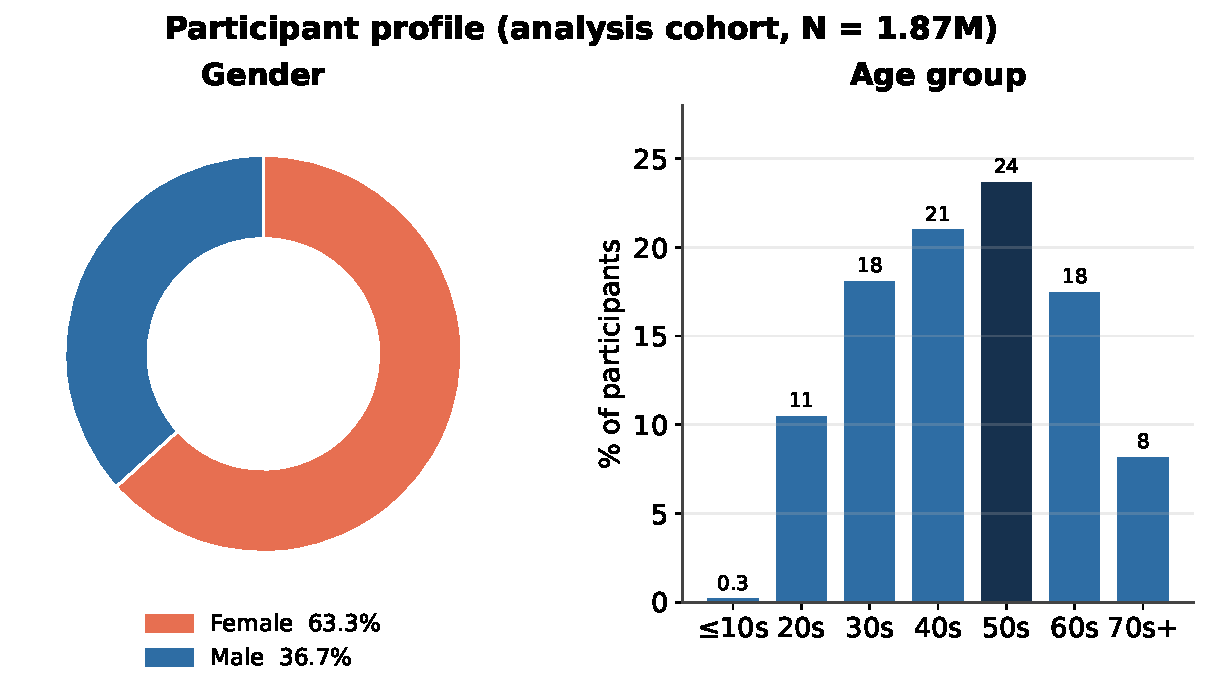
\includegraphics[width=0.9\linewidth]{fig_profile.pdf}\\[0.2em]
  {\footnotesize \hi{63\%} of members are women; participation peaks in the \textbf{40s--50s}, with strong representation into the 60s.}
\end{frame}

\begin{frame}{Daily activity: men out-step women; both peak in their 60s}
  \centering
  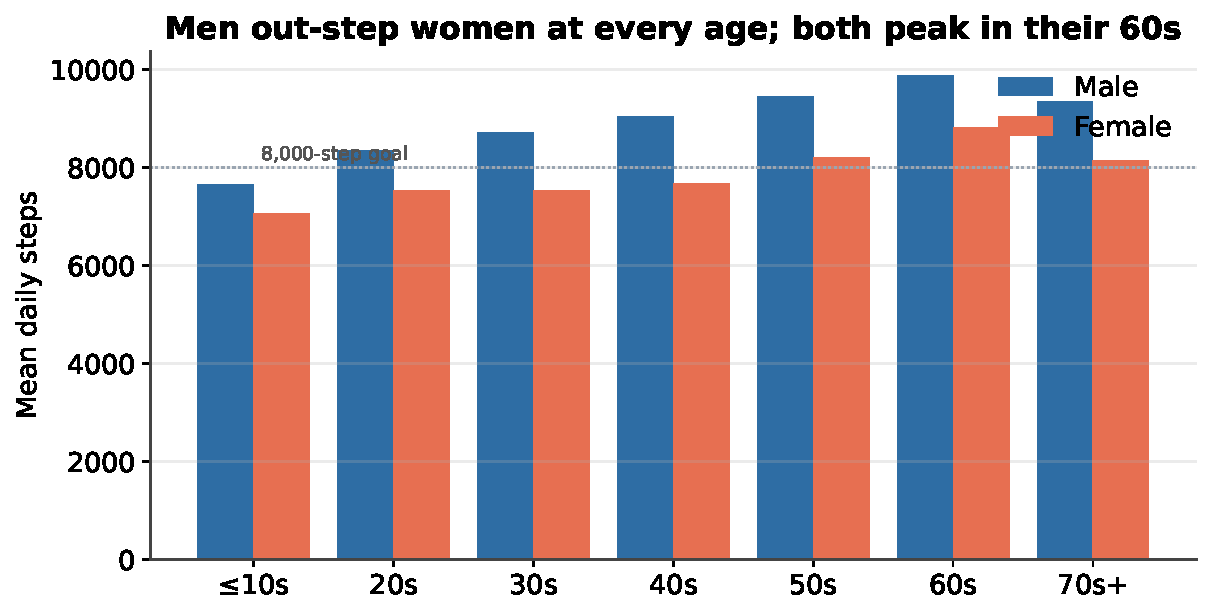
\includegraphics[width=0.82\linewidth]{fig_steps_gender_age.pdf}\\[0.2em]
  {\footnotesize Despite a lower sign-up rate, \hc{men average $\sim$15\% more steps} (9{,}238 vs 8{,}014/day). Steps rise with age to a peak in the \textbf{60s}, easing slightly at 70+.}
\end{frame}

\begin{frame}{Weekly rhythm: a pronounced weekend slump}
  \centering
  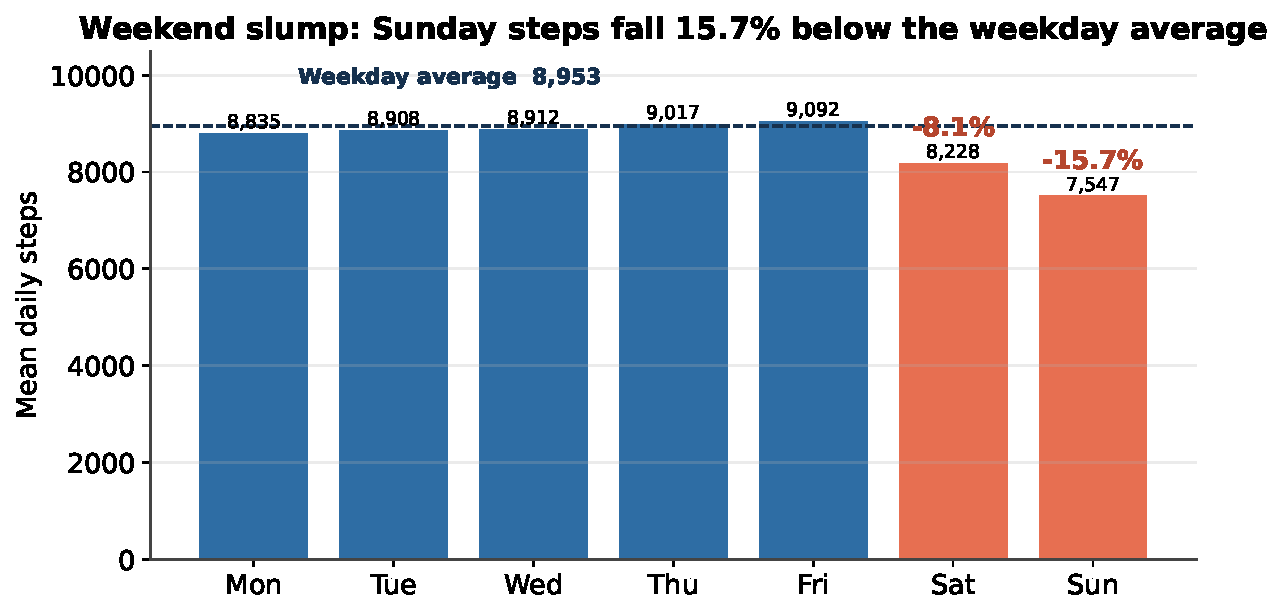
\includegraphics[width=0.82\linewidth]{fig_weekday_steps.pdf}\\[0.2em]
  {\footnotesize Activity is \textbf{weekday-anchored}: Sunday steps fall \hc{15.7\%} below the weekday average. Participation and goal achievement dip on weekends too.}
\end{frame}

\begin{frame}{Holidays: the steepest dips of all}
  \centering
  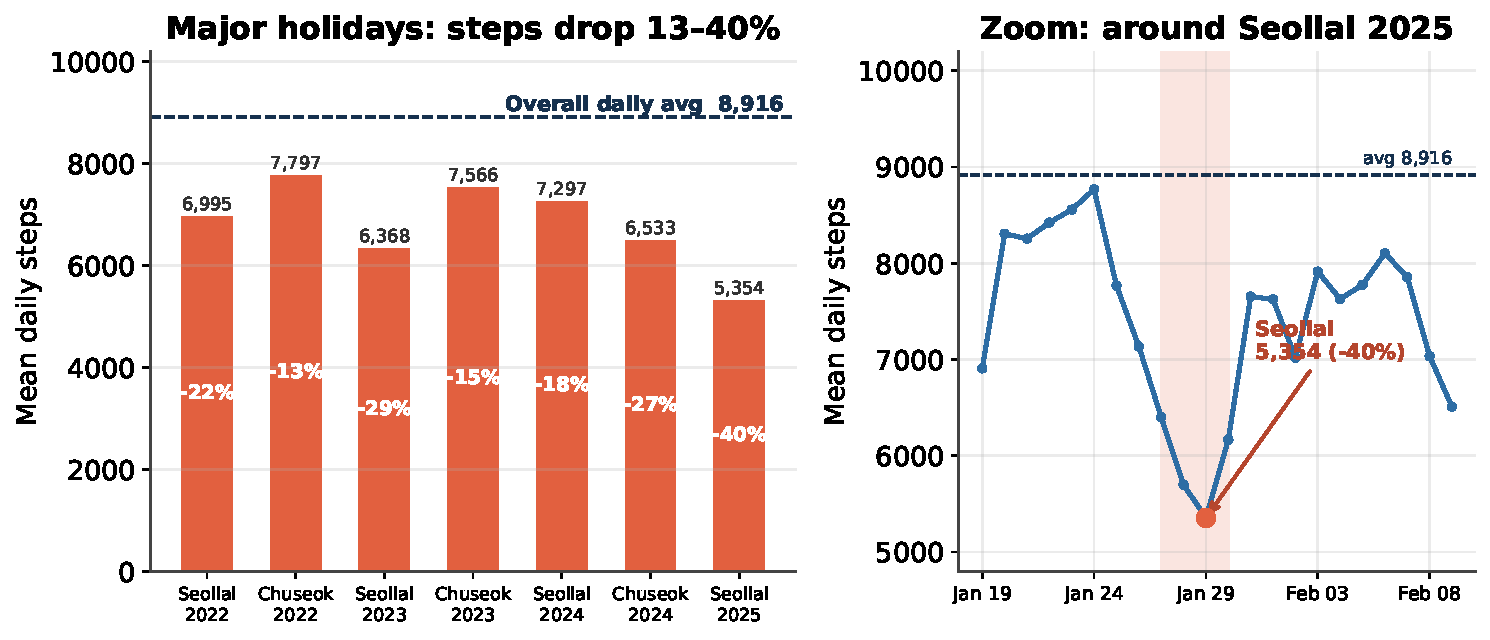
\includegraphics[width=0.92\linewidth]{fig_holidays.pdf}\\[0.2em]
  {\footnotesize Korea's major holidays --- \textbf{Seollal} (Lunar New Year) and \textbf{Chuseok} --- bring far larger drops than weekends: \hc{13--40\%} below the overall daily average on the holiday itself, with Seollal 2025 the single lowest day in the record (5{,}354 steps, $-40\%$).}
\end{frame}

\begin{frame}{Engagement over time: $\sim$40\% stay ``active''}
  \centering
  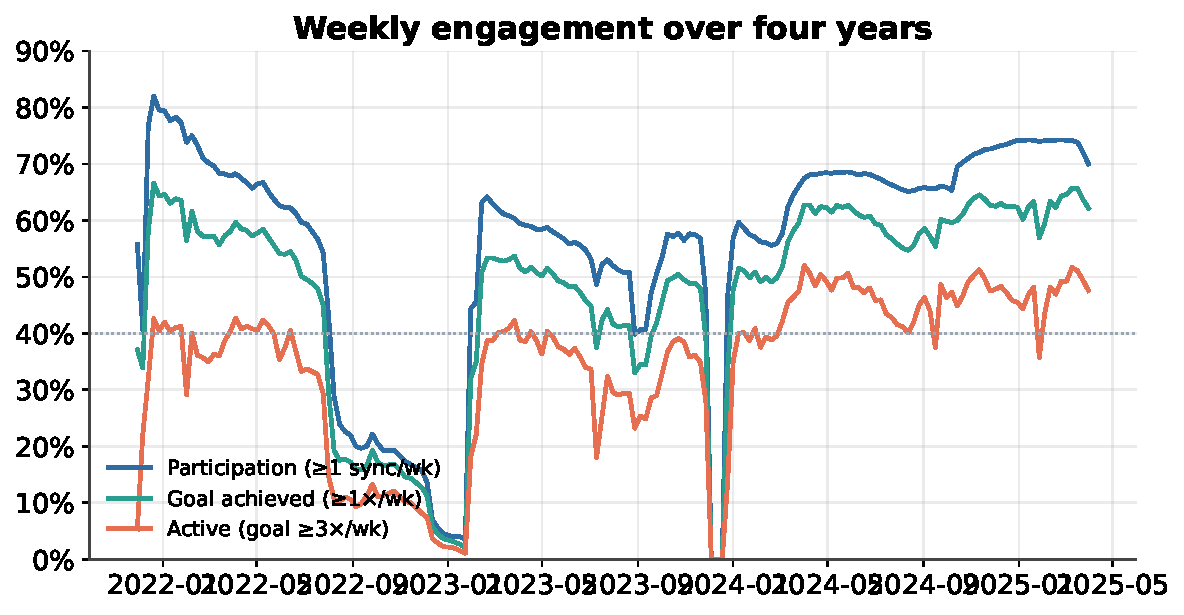
\includegraphics[width=0.82\linewidth]{fig_engagement_ts.pdf}\\[0.2em]
  {\footnotesize After each enrollment wave, engagement settles into a steady regime: $\sim$70\% participate weekly, $\sim$60\% hit the goal weekly, and \hc{$\sim$40--45\% remain active} ($g\!\ge\!3$/week).}
\end{frame}

\begin{frame}{Engagement rises steadily with age}
  \centering
  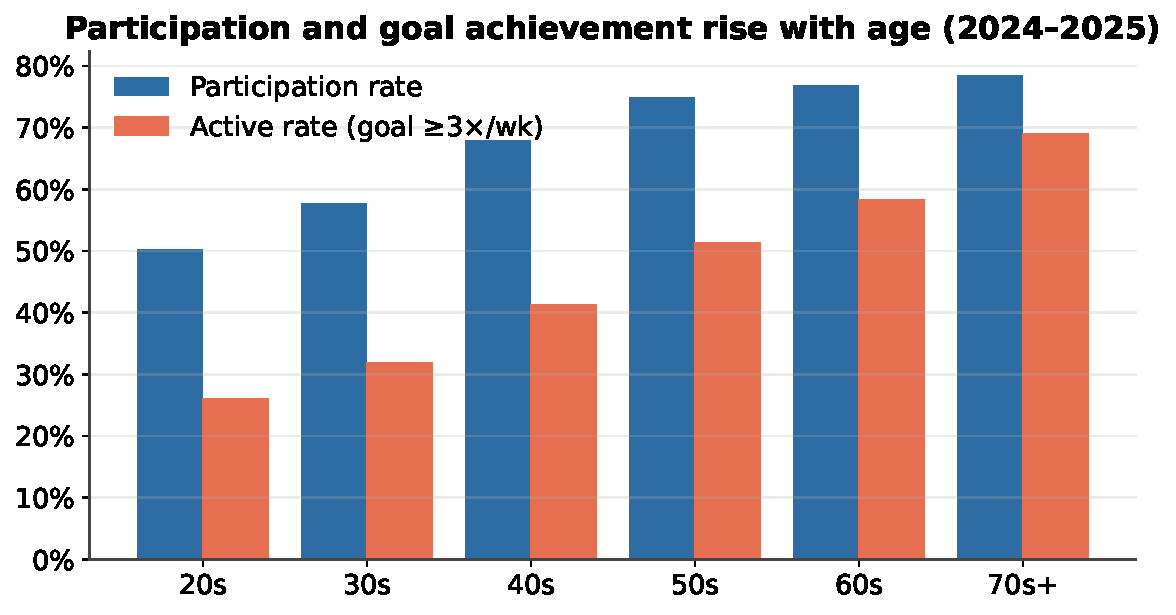
\includegraphics[width=0.82\linewidth]{fig_part_goal_by_age.pdf}\\[0.2em]
  {\footnotesize Older members are \emph{more} engaged: both participation and the active rate climb monotonically from the 20s to the 70s. Younger members are the hardest to retain.}
\end{frame}

\begin{frame}{Retention: older participants persist far longer}
  \centering
  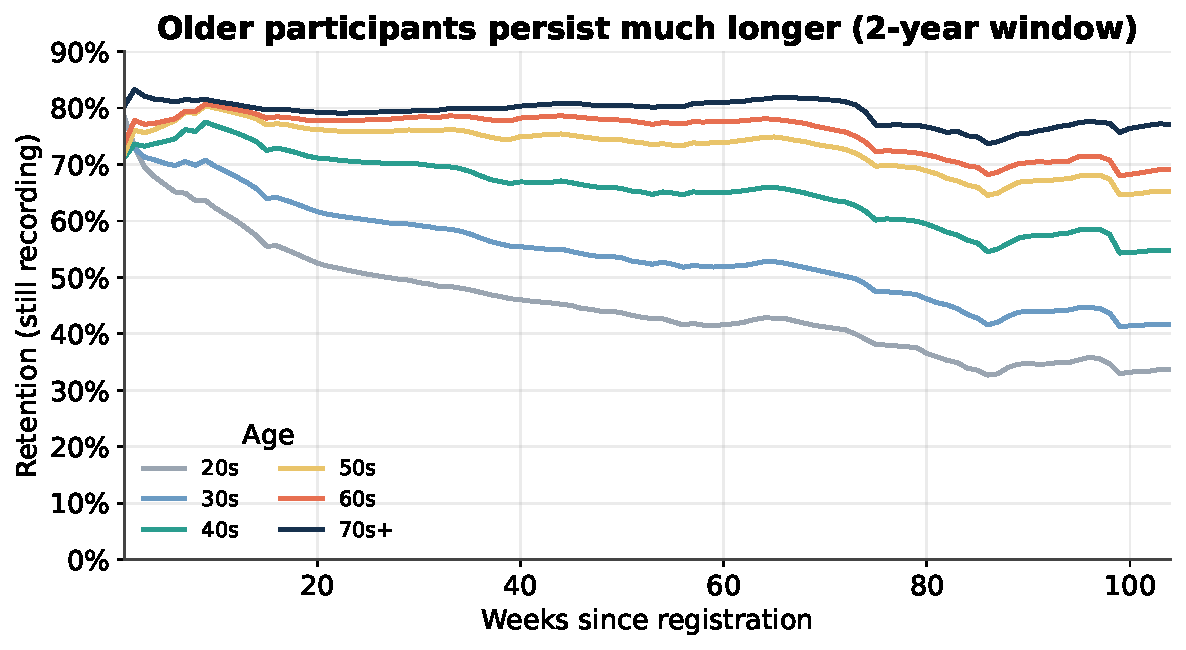
\includegraphics[width=0.82\linewidth]{fig_retention.pdf}\\[0.2em]
  {\footnotesize Two years after joining, retention ranges from \hc{$\sim$4\%} (20s) to \hc{$\sim$24\%} (60s). Persistence increases with age across the entire follow-up.}
\end{frame}

\begin{frame}{Regional variation is modest across Seoul}
  \centering
  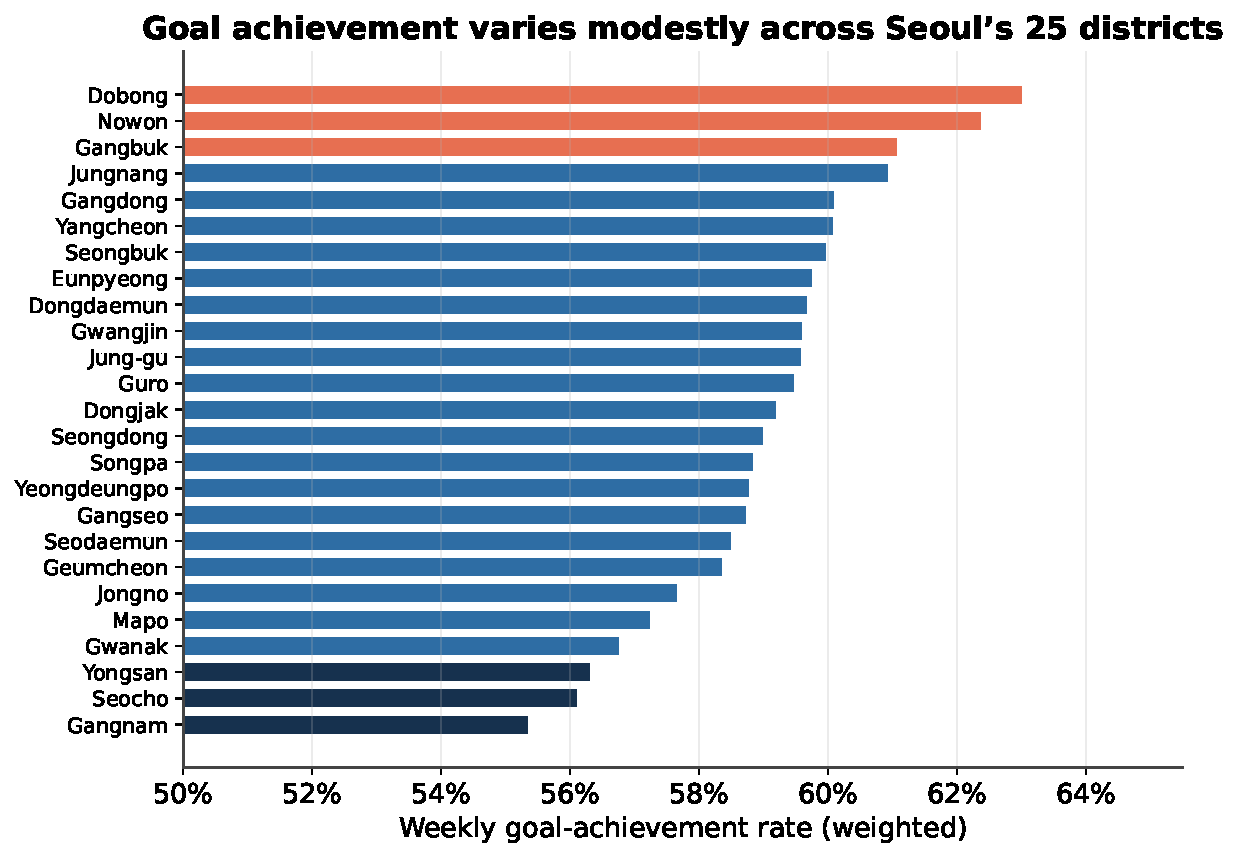
\includegraphics[width=0.62\linewidth]{fig_district.pdf}\\[0.1em]
  {\footnotesize Weekly goal-achievement spans only $\sim$55--63\% across all 25 districts --- engagement is fairly even city-wide, with a mild edge for several outer-northern districts.}
\end{frame}

% #####################################################################
\begin{frame}{Dropout is recoverable --- especially for once-active members}
  \centering
  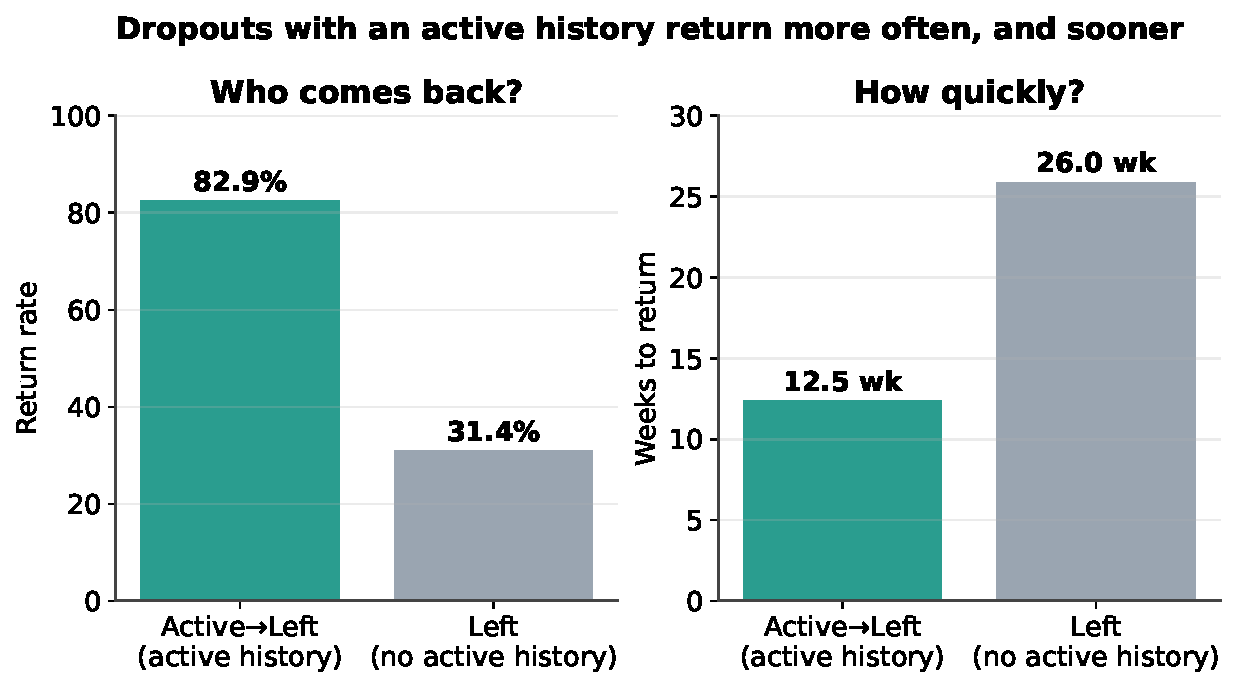
\includegraphics[width=0.78\linewidth]{fig_segments.pdf}\\[0.2em]
  {\footnotesize Members active before lapsing (\textbf{Active\,$\to$\,Left}) return at \hc{82.9\%} (vs 31.4\%) and \textbf{twice as fast} (12.5 vs 26.0 weeks). A history of activity is the strongest signal of return.}
\end{frame}

% #####################################################################
\section{Findings \& implications}
% #####################################################################

\begin{frame}{Key findings}
  \begin{enumerate}
    \item \textbf{Scale works.} A municipal mHealth program reached \hi{2.18M} members, with a \hi{1.6M} active base.
    \item \textbf{Sign-up $\neq$ intensity.} Women join more (63\%), but men average $\sim$15\% more steps.
    \item \textbf{Age is protective.} Engagement, goal achievement and retention all \textbf{rise with age}; younger members churn fastest.
    \item \textbf{Habits are weekday-anchored.} A consistent \hc{$-15.7\%$} Sunday slump.
    \item \textbf{Activity sustains.} $\sim$40--45\% stay active ($g\!\ge\!3$/week) in steady state.
  \end{enumerate}
\end{frame}

\begin{frame}{Implications \& future work}
  \begin{columns}[T]
    \begin{column}{0.5\textwidth}
      \textbf{\color{ink}Policy already moved this way}
      \begin{itemize}
        \item Late 2025 (after our data window), the program added a \textbf{weekend rule}: miss the step goal on \emph{both} weekend days and the \textbf{weekly bonus is withheld}.
        \item This directly targets the \hc{weekend slump} we document --- our descriptive finding aligns with a real policy change.
      \end{itemize}
      \vspace*{0.3em}
      \textbf{\color{ink}Other design levers}
      \begin{itemize}
        \item Protect early retention of \textbf{younger / short-tenure} members.
        \item Leverage older adults as a built-in retention success.
      \end{itemize}
    \end{column}
    \begin{column}{0.5\textwidth}
      \textbf{\color{ink}Future analysis}
      \begin{itemize}
        \item \textbf{Link step data to health records.} We used step data only; joining clinical / check-up data at scale could test whether \emph{sustained} activity improves health --- now feasible as the panel lengthens (early waves were too short before).
        \item \textbf{Mental-health outcomes.} Higher daily step counts are linked to fewer depressive symptoms (e.g.\ +1{,}000 steps/day $\approx$ 9\% lower depression risk; Bizzozero-Peroni et al., \textit{JAMA Netw Open} 2024) --- a natural extension for this population.
        \item \textbf{Effectiveness \& equity}: pre/post step change; deeper district / enrollment-type analysis.
      \end{itemize}
    \end{column}
  \end{columns}
\end{frame}

% ----------------------------- THANKS --------------------------------
\begin{frame}[standout]
  Thank you
  \vspace{0.6em}

  {\normalsize Questions \& discussion welcome}
  \vspace{1.2em}

  {\footnotesize Youngdoo Jeong \,\textbullet\, Dept.\ of Statistics, University of Seoul \\[0.2em]
  JSM 2026 \,\textbullet\, Session 3028}
\end{frame}

% #####################################################################
\appendix
% #####################################################################

\begin{frame}{Appendix --- Segment definitions in detail}
  {\footnotesize Early-window features (first $\approx$9 weeks) used to construct the segments. ``Active'' uses the goal-$\ge$3-days/week rule; ``churn / return'' is based on a sustained recording gap and any subsequent re-recording.}
  \vspace*{0.6em}
  \centering\footnotesize
  \renewcommand{\arraystretch}{1.25}
  \begin{tabular}{@{}l r r r r@{}}
    \toprule
    Segment & Early active-week share $\rho$ & Avg.\ goal-days/wk & Weeks-before-churn & Return rate / time\\
    \midrule
    Active            & 0.74 & 4.29 & --   & --\\
    Normal            & 0.27 & 1.61 & --   & --\\
    Left              & 0.15 & 0.87 & 26.7 & 31.4\% / 26.0 wk\\
    Active\,$\to$\,Left & 0.29 & 1.64 & 33.9 & \hc{82.9\%} / \hc{12.5\,wk}\\
    \bottomrule
  \end{tabular}
  \vfill
  {\color{graytx}\scriptsize ``--'' : not applicable (Active / Normal do not churn by construction). Figures are segment means over the analysis cohort.}
\end{frame}

\end{document}
